\cotefile{36}

\scanpage{65}

\margin{\fbox{$\delta\overset{\unsure{\mathrm{dfn}}}{=}\operatorname{Im}(\operatorname{Pic}(X_0)\longrightarrow\underline{\operatorname{NS}}_{X_0/k}(k))$}}
\uline{Théorème}\quad $S$ trait str. local

$X$ schéma propre sur $S$, régulier, tel que $\underline O_S\xrightarrow{\sim}f_*(\underline O_X)$, et que $X_\eta$ admette \inserted{un 0-cycle de degré 1}

$\Delta$ le groupe des diviseurs sur $X$ tels que $\operatorname{supp.}\Delta\subset X_0$
\[
c:\Delta\longrightarrow\deleted{\unsure{\operatorname{NS}(X_0)}}=\underline{\operatorname{NS}}\deleted{\unsure{{}_{X_0/k}(k)}}\inserted{(X_0)}
\]
défini comme composé
\diagram{\begin{tikzcd}[column sep=small]
\Delta\arrow[r]&\operatorname{Pic}(X)\arrow[r]&\operatorname{Pic}(X_0)\arrow[r]&\underline{\operatorname{Pic}}_{X_0/k}(k)\arrow[r,dash]&\underline{\operatorname{NS}}_{X_0/k}(k)\arrow[r]&N
\end{tikzcd}}
\[
\left\{\begin{gathered}
\delta=\deleted{\unsure{\operatorname{Coker}c\text{ qui}}}\ \text{ss-grpe de torsion de }\operatorname{Coker}c,\\
\deleted{\unsure{\operatorname{NS}\text{ et }Z}\ \unsure{\text{qui est le}}\ \unsure{\text{de}}\delta\ \unsure{\text{dans}}\ \underline{\operatorname{NS}}(X_0),\ \text{de sorte que }\Delta\longrightarrow\Lambda\xrightarrow{\lambda}\delta\longrightarrow0}
\end{gathered}\right.
\]
\deleted{\unsure{Supposons}} Alors $\delta$ est un grpe \uline{fini}\unsure{;|,} \inserted{\deleted{\unsure{torsion de}} $\unsure{{}_t|T}\operatorname{NS}(X_0)=\delta'$, soit $\delta''=\delta/\delta'$} et pour tout entier $n$ premier à $p$, on a une suite exacte canonique
\diagram{\begin{tikzcd}[column sep=tiny,row sep=small]
&&&\inserted{{}_n\delta/{}_n\delta'\ \deleted{\longrightarrow\delta''}}&&&&\\
(*)\quad\unsure{0}\arrow[r,dash]&H^1(X,\mu_n)\arrow[r,"u_n"]\arrow[d,phantom,"\unsure{\Vert|\wr}" description]&H^1(X_{\bar\eta},\mu_n)^I\arrow[r]\arrow[ur,bend left=20]&\deleted{{}_n\delta''}\arrow[r]&\deleted{\unsure{\delta'}}\delta'_n\arrow[r]&\delta_n\arrow[r]&\delta''_n\arrow[r]&0\\
&\inserted{H^1(X_0,\mu_n)}&&\deleted{\unsure{\delta'}}&&&&
\end{tikzcd}}
compatible avec les morphismes de transition évidents en $n$, d'où par passage à la limite, pour tt $\ell$ nb. pr. $\neq p$
\[
H^1(X,\mathbb Z_\ell)\xrightarrow{\sim}H^1(X_{\bar\eta},\mathbb Z_\ell)^I
\]
(\uline{Théorème des cycles invariants}).
\margin{(\unsure{car|cas} $X$ i}

\uline{Dém} $X$ est plat sur $S$, donc $X_\eta$ dense \unsure{ds|dans} $X$, et $H^1(X,\mu_n)\hookrightarrow H^1(X_\eta,\mu_n)$. On \unsure{trouve|donc} le \unsure{diagramme|diag. commut}
\diagram{\begin{tikzcd}[column sep=small,row sep=large]
H^1(X,\mu_n)\arrow[r,"\substack{\alpha\\\sim}"]\arrow[d]&{}_n\operatorname{Pic}(X)\arrow[d]&&\\
H^1(X_\eta,\mu_n)/(\mathbb Z/n\mathbb Z)\arrow[r,"\substack{\alpha_\eta\\\sim}"]\arrow[d]&{}_n\operatorname{Pic}(X_\eta)\arrow[r,"\substack{\beta_\eta\\\sim}"]\arrow[d]&{}_nP(K)\arrow[r,phantom,"\simeq" description]\arrow[d]&{}_nP(\bar K)^I\arrow[dl,bend left=20]\\
H^1(X_{\bar\eta},\mu_n)\arrow[r,"\substack{\alpha_{\bar\eta}\\\sim}"]&{}_n\operatorname{Pic}(X_{\bar\eta})\arrow[r,"\substack{\beta_{\bar\eta}\\\sim}"]&{}_nP(\bar K)&
\end{tikzcd}}
où $\alpha,\alpha_\eta,\alpha_{\bar\eta}$ sont des isom par \deleted{\unsure{suite exacte}} de Kummer et $f_*(\underline O_X)\simeq\underline O_S$ (\uline{NB} $V^*/V^{*n}=0$, $K^*/K^{*n}=\mathbb Z/n\mathbb Z$, car $V$ \uline{str.} local) $\beta_\eta$ (et $\beta_{\bar\eta}$) \unsure{sont} isom à cause de l'existence d'un 0-cycle de degré 1 sur $X_\eta$, donc on voit que $u_n$ \unsure{de|dans} (*) s'identifie:
\[
(**)\qquad{}_n\unsure{v|\nu}:\quad{}_n\operatorname{Pic}(X)\longrightarrow{}_n\operatorname{Pic}(X_\eta)
\]
Comme $X$ est régulier (il suffirait: anneaux locaux factoriels) on a
\diagram{\begin{tikzcd}
0\arrow[r]&\Gamma\arrow[r,"i"]&\operatorname{Pic}(X)\arrow[r,dash,"\unsure{v|\nu}"]&\operatorname{Pic}(X_\eta)\arrow[r]&0
\end{tikzcd}}
où $\Gamma=\Delta/\mathbb Z\cdot X_0$, d'où
\[
\operatorname{Coker}u_n\simeq\operatorname{Coker}\unsure{{}_nv_n|{}_n\nu_n|{}_nv|{}_n\nu}\unsure{\simeq|=}\operatorname{Ker}i_n,\quad\text{où }i_n:\Gamma_n\longrightarrow\operatorname{Pic}(X)_n
\]

\margin{64}

\scanpage{66}
\mspage{- 10 -}
\margin{n° 384}
$\mathfrak M_+(G)$ (ch. IV, § 1, n° 1, prop. 4) et l'ensemble des $\alpha\in T$ telles que $\alpha(U)\leq 1$ est donc fermé. Il en résulte que l'ensemble $\Delta_U$ des $\alpha\in T$ satisfaisant à $\alpha(\{e\})\geq 1$ et à $\alpha(U)\leq 1$ est \uline{fermé} : remarquons que ces conditions sont équivalentes à $\alpha(\{e\})=\alpha(U)=1$ et par suite, $\Delta_U$ se compose exactement de l'\uline{ensemble des mesures de Haar normalisées des sous-groupes discrets} $H$ \uline{tels que} $H\cap U=\{e\}$ ; nous noterons $D_U$ l'ensemble de ces sous-groupes discrets.

Soit maintenant $\varphi$ une fonction de $\mathcal K_+(G)$, de support contenu dans $U$ et telle que $\varphi(e)=1$ : on a alors $\alpha(\varphi)=1$ pour toute $\alpha\in\Delta_U$, ce qui montre que $\Delta_U$ est contenu dans le \uline{compact} $T\cap L_\varphi$ (prop. 2) et est donc lui-même \uline{compact}. L'application canonique de $\Delta_U$ sur $D_U$ est donc un homéomorphisme et on a :

PROPOSITION 7.- \uline{Pour tout voisinage ouvert} $U$ \uline{de} $e$, \uline{l'ensemble} $D_U$ \uline{des sous-groupes discrets} $H$ \uline{de} $G$ \uline{tels que} $H\cap U=\{e\}$ \uline{est compact}.

Soit maintenant $V$ un autre voisinage ouvert de $e$, relativement compact et tel que $\overline V\subset U$ et soit $\varphi\in\mathcal K_+(G)$, de support contenu dans $U$ et avec $\varphi(x)=1$ pour $x\in V$. On a $\alpha(\varphi)=1$ pour $\alpha\in\Delta_U$ et il existe donc un voisinage $W$ de $\alpha$ dans $\Delta$ tel que $\beta(\varphi)<2$ pour $\beta\in W$ : on a alors $W\subset\Delta_V$, ce qui montre que $\Delta_V$ est un voisinage de $\Delta_U$. Par suite, les \uline{intérieurs} des sous-espaces $\Delta_U$ de $\Delta$ forment un recouvrement ouvert de $\Delta$ par des ensembles relativement compacts. On en déduit (compte tenu de ce que $\Delta_{U_1}\cap\cdots\cap\Delta_{U_n}=\Delta_{U_1\cap\cdots\cap U_n}$) :

PROPOSITION 8.- \uline{Le sous-espace} $\Delta$ \uline{de} $T$ \uline{est localement compact ; pour qu'une partie} $A$ \uline{de} $\Delta$ \uline{soit relativement compacte, il faut et il suffit qu'il existe un voisinage ouvert} $U$ \uline{de} $e$ \uline{tel que} $A\subset\Delta_U$.

Supposons maintenant que $G$ satisfasse à la condition suivante :

(L)\qquad il existe un voisinage $Q$ de $e$ tel que le seul sous-groupe \uline{discret} de $G$ contenu dans $Q$ soit le sous-groupe réduit à $\{e\}$.

En termes imagés, la condition (L) signifie que $G$ n'a pas de sous-groupes discrets arbitrairement petits. * On peut montrer que tout groupe de Lie satis-
\margin{65}

\scanpage{67}
\deleted{\unsure{Comme|Corol}}
\deleted{On sait que}
\deleted{On sait que}

On a d'autre part, si
\[
\deleted{\unsure{0|\cdot}\unsure{\longrightarrow|\mathbin{-}}\Gamma\longrightarrow}\qquad \unsure{j_0|j_a}:\Gamma\longrightarrow\operatorname{Pic}(X_0)\qquad\deleted{\unsure{est|\longrightarrow}}
\]
est le composé, d'où des $j_n:\Gamma_n\mathbin{-}\operatorname{Pic}(X_0)_n$, \deleted{\unsure{donc} \unsure{l'inclusion}} \inserted{\unsure{on a}} l'inclusion \unsure{évidente|evidente}\unsure{:|;}
\[
\operatorname{Ker}i_n\subset\operatorname{Ker}j_n
\]
\margin{\uline{Lemme.} $\operatorname{Pic}(X)_n\hookrightarrow\operatorname{Pic}(X_0)_n$ (du moins si $S$ complet, ce qui suffit pour le th.) faisable par la rigidité}
Cette inclusion est \inserted{en fait} une \uline{identité}. Pour le voir, on note que si $\underline L$ est un faisceau inv. sur $X$, et si $\underline L_n=\underline L|X_n$ est \unsure{écrit|écris} comme puissance $n$ième, alors l'obstruction à écrire $\underline L_{n\unsure{+}1}$ comme puissance $n$ième est nulle (cf \unsure{FGA|PCA}, exposé sur Picard). On a d'autre part
\[
\operatorname{Pic}(X_0)=\underline{\operatorname{Pic}}_{X_0/k}(k)
\]
grâce au fait que $X_0$ a un $0$-cycle de degré $1$, d'où
\diagram{\begin{tikzcd}[column sep=large]
0\arrow[r,dash]&\operatorname{Pic}^{0}(X_0)\arrow[r,dash]\arrow[d,equal,"\mathrm{dfn}"']&\operatorname{Pic}(X_0)\arrow[r]&\operatorname{NS}(X_0)'\arrow[r]\arrow[d,equal,"\mathrm{dfn}"']&0\\
&\underline{\operatorname{Pic}}^{0}_{X_0/k}(k)&&\operatorname{Im}\bigl(\underline{\operatorname{Pic}}_{X_0/k}(k)\longrightarrow\underline{\operatorname{NS}}_{X_0/k}(k)\bigr)
\end{tikzcd}}
et $\operatorname{Pic}^{0}(X_0)$ est $n$-divisible, donc on a
\[
\operatorname{Pic}(X_0)_n\hookrightarrow\operatorname{NS}(X_0)_n
\]
\margin{\uline{joindre au lemme précédent}}
donc si
\[
\unsure{k}:\Gamma\longrightarrow\operatorname{NS}(X_0)
\]
est le composé $\Gamma\xrightarrow{j}\operatorname{Pic}(X_0)\longrightarrow\operatorname{NS}(X_0)$, on trouve
\[
\operatorname{Coker}u_n\simeq\operatorname{Ker}\unsure{k_n}
\]
Je dis que \inserted{$\Gamma$ \uline{est sans torsion et que}} $\delta$ est \uline{injectif} i.e. qu'un faisceau inv. sur $X$ qui est banal sur $X_\eta$, et qui sur $X_0$ est \inserted{num. équiv.} \deleted{\inserted{(comme \illegible{1} \unsure{de} torsion)}} à zéro, est trivial.
\margin{cf plus bas une démonstration}
\deleted{L'hyp. que l'image}
\deleted{$\unsure{L'\in\operatorname{Pic}(X)}$ \unsure{dans} $\operatorname{NS}(X_0)$ est nulle \deleted{\unsure{implique}} \inserted{\unsure{implique}} \deleted{\unsure{par le}} \unsure{indique|implique} (par rigidité) que que $\underline L$ est \unsure{inft|infiniment} $\ell$-divisible pour tt $\ell\ne p$, et on peut faire la division de façon \underline{unique}, en restant dans}
\unsure{finalt|finalement} il est banal, on trouve
une suite exacte
\deleted{\unsure{k|\xi}}
\deleted{\diagram{\begin{tikzcd}
\unsure{0|\cdot}\arrow[r,dash]&\Gamma\arrow[r,"\unsure{k}",dash]&\operatorname{NS}(X_0)'\arrow[r]&\unsure{\delta|\operatorname{Coker}k}\arrow[r]\arrow[d,equal]&0\\
&&&\operatorname{Coker}\unsure{k}\unsure{=\operatorname{Coker}|=}\unsure{\Delta|\delta}
\end{tikzcd}}}
\deleted{\inserted{$\operatorname{Coker}k=\operatorname{Coker}\Delta$}}
\margin{\inserted{\diagram{\begin{tikzcd}[column sep=small]
0\arrow[r]&\Gamma\arrow[r,"k'"]&\operatorname{NS}(X_0)'\arrow[r,"\lambda"]\arrow[d,equal]&\delta\arrow[r]&0\\
&&\text{\unsure{ss-grpe|ss-groupe} \unsure{des|de} }\operatorname{NS}(X_0)\text{ dont un multiple tombe ds }\Gamma
\end{tikzcd}}}}
d'où \inserted{par} \unsure{la|le} suite exacte habituelle
\[
\deleted{\unsure{\operatorname{Coker}|donc}}\quad \operatorname{Ker}k_n=\operatorname{Ker}k'_n\simeq\operatorname{Coker}{}_n\lambda
\]
Comme $\Gamma$ est sans torsion, \deleted{\unsure{donc|on}} $\delta'\xrightarrow{\lambda}\delta$ est injectif, et on trouve que $\operatorname{Coker}{}_n\lambda={}_n\delta/{}_n\delta'$. On termine grâce à la suite
\margin{66}

\scanpage{68}
\mspage{- 9 -}
\margin{n° 384}
Puisque $Q_\alpha$ est compact, la constante 2 appartient à $\mathcal K_+(Q_\alpha)$ et il existe une fonction $g\in\mathcal K_+(G)$ avec $g*\alpha(x)=2$ pour tout $x\in G$. Soit $K$ le support de $g$ et posons $L=DK$. Il existe un voisinage $W$ de $\alpha$ dans $T^\circ$ tel que $g*\beta(x)\geq 1$ pour $x\in L$ et $\beta\in W$. Soit $\beta\in W$. Comme le support de $g*\beta$ est contenu dans $KH_\beta$, on a donc $DK\subset KH_\beta$. Supposons démontré que $D^{r-1}K\subset KH_\beta$ : on a alors :
\[
(14)\qquad D^rK=DD^{r-1}K\subset DKH_\beta\subset KH_\beta H_\beta=KH_\beta.
\]
Comme $G$ est la réunion des $D^r$, on en déduit que $G=KH_\beta$. De plus, on a $g*\beta\geq 1$ sur $K$ et $g*\beta$ est invariante à droite par $H_\beta$ : on a donc $g*\beta\geq 1$ partout et ceci montre que $W\subset T^\circ(g)$. Donc $T^\circ(g)$ est bien un voisinage de $\alpha$ et il est clair que $\beta\in T^\circ(g)$ entraîne $G=KH_\beta$ et par suite que $G/H_\beta$ est compact.

COROLLAIRE 1.- \uline{L'ensemble} $T^c$ \uline{des} $\alpha\in T^\circ$ \uline{telles que} $G/H_\alpha$ \uline{soit compact est un ouvert de} $T^\circ$ \uline{et la restriction de} $v$ \uline{à} $T^c$ \uline{est continue}.

COROLLAIRE 2.- \uline{L'ensemble} $S^c$ \uline{des sous-groupes fermés unimodulaires à quotient compact est un sous-ensemble ouvert de l'ensemble compact} $S^\circ$ \uline{des sous-groupes} \inserted{\uline{fermés unimodulaires}.}

La proposition 6 n'est pas exacte si on ne suppose pas que $G$ est engendré par un compact (exer.\ ).

7. \uline{Sous-groupes discrets.}

Soit $D$ le sous-espace de $S$ formé des sous-groupes \uline{discrets} de $G$ et soit $\Delta$ le sous-espace de $T$ formé des mesures de Haar \uline{normalisées} des éléments de $D$ : pour qu'un élément $\alpha\in T$ appartienne à $\Delta$, il faut et il suffit que $\alpha(\{e\})=1$. On a évidemment $D\subset S^\circ$ et $\Delta\subset T^\circ$.

Pour tout compact $K$ de $G$, l'application $\alpha\longrightarrow\alpha(K)$ est semi-continue \uline{supérieurement} sur $\mathfrak M_+(G)$ (ch. IV, § 4, n° 4, Remarque). Par suite l'ensemble des $\alpha\in T$ telles que $\alpha(\{e\})\geq 1$ est \uline{fermé} dans $T$. D'autre part, pour tout voisinage ouvert $U$ de $e$, l'application $\alpha\longrightarrow\alpha(U)$ est semi-continue inférieurement sur
\margin{67}

\scanpage{69}
exacte
\[
0\mathbin{-}\delta'\mathbin{-}\delta\mathbin{-}\delta''\mathbin{-}0
\]
et la suite exacte associée
\[
0\mathbin{-}{}_n\delta'\mathbin{-}{}_n\delta\mathbin{-}{}_n\delta''\mathbin{-}\delta'_n\mathbin{-}\delta_n\mathbin{-}\delta''_n
\]
Reste : prouver : \textcircled{\unsure{a|0}}) le fait que $\Gamma$ est sans torsion. Mais $\Gamma=\mathbf Z/d\mathbf Z$, \unsure{où|i.e.|:=} $d$ est le pgcd des $d_i$, $X_0=\sum d_iD_i$, \& $X_{0\mathrm{red}}=\sum\unsure{D_i}$. \deleted{(On \unsure{voit|sait} que si $\exists$ sur $X$ un $0$-cycle \unsure{un} $0$-cycle de degré $1$} si on a un pt fermé $x$ de $X_\eta$, son adhérence \inserted{schématique dans $X$} est un sous-schéma \inserted{fermé $Z$} \deleted{plat} de $X$, plat et fini sur $S$, \deleted{qui est} dont le degré sur $S$ est aussi égal à la multiplicité d'intersection \inserted{$Z.X_0$} sur $X$, qui est $\sum d_iZ.D_i$, donc multiple de $d$. Donc si $d'\deleted{\unsure{d}}$ est le pgcd des degrés des 0-cycles sur $X_\eta$, on a $d\mid d'$. Comme $d'=1$, on a $d=1$.
\margin{donner \uline{lemme} (ici \unsure{sans|sur} $X$ régulier, semble-t-il)}

\textcircled{b} $\Gamma\longrightarrow\operatorname{NS}(X_0)$ est \uline{injectif}.
\margin{\uline{Donner cor. Néron} \uline{ou th.}}
[Soit $R$ son noyau, \inserted{qui est $\mathbf Z$-libre de t.f. \unsure{p. $0$|$r=0$|$\ne0$})}, \deleted{\unsure{On}} a des suites exactes
\[
0\mathbin{-}\mathrm H^1(X,\mu_n)\mathbin{-}\mathrm H^1(X_{\bar\eta},\mu_n)^I\unsure{\mathbin{-}|\longrightarrow}{}_{\unsure{n|a}}\Gamma_n\mathbin{-}\operatorname{NS}(X_0)_n
\]
d'où, par passage à la limite sur les puissances d'un $\ell$
\[
0\mathbin{-}\mathrm H^1(X,\mathbf Z_\ell(1))\mathbin{-}\mathrm H^1(X_{\bar\eta},\mathbf Z_\ell(1))^I\longrightarrow\deleted{T_\ell}(\Gamma\deleted{\unsure{)}}\otimes\mathbf Z_\ell\mathbin{-}\deleted{T_\ell}(\operatorname{NS}(X_0)\deleted{\unsure{)}}\otimes\mathbf Z_\ell
\]
i.e. on trouve, comme $\deleted{T_\ell(R)}\unsure{\deleted{\simeq}|\simeq}R\otimes\mathbf Z_\ell\simeq\operatorname{Ker}(\Gamma\otimes\mathbf Z_\ell\mathbin{-}\operatorname{NS}(X_0)\otimes\mathbf Z_\ell)$
\deleted{$T_\ell(R$}\quad$\unsure{\beta|\rho}$
\[
0\mathbin{-}\mathrm H^1(X,\mathbf Z_\ell(1))\mathbin{-}\mathrm H^1(X_{\bar\eta},\mathbf Z_\ell(1))^I\mathbin{-}R\otimes\mathbf Z_\ell\mathbin{-}0
\]
Donc notre assertion équivaut à dire que l'on a la formule des cycles invariants ; \deleted{\unsure{cette|c'est}} il suffit \unsure{$\subset$|c.} de la prouver à torsion près.]
\margin{[\quad] en remarque après le cor.}

\deleted{L'idée est de se ramener au cas où $X$ est de dim relative un. Dans ce cas, on \uline{sait} que $\Gamma$ est nul (c'est le fait que une certaine matrice \inserted{d'intersection $(D_i.D_j)$} est de rang $\deleted{\unsure{\ell|r|(}}r-1)$, où $r$ est le nb de composantes $D_i$)}
Or c'est fait par Raynaud dans sa note : \unsure{s|S}pécialisation des foncteurs de Picard, \uline{th. 3} --- dans version sans \deleted{\unsure{dans|l'hyp.}} hyp. projective.
\margin{donner dém. directe \unsure{au|en} cas de dim. rel. 1}
\deleted{[Il \unsure{faut} \unsure{que} \unsure{l'on} \unsure{suppose} que $R^{\unsure{1|I}}_{\unsure{X,\Lambda}}$ \unsure{est fini} \unsure{si} $\unsure{d}=\unsure{f|p}$,
\unsure{des} \illegible{1} \unsure{comme} \unsure{cas} \unsure{du|de} \illegible{1} $\operatorname{NS}(X_0)$ \unsure{est nul}, \illegible{1} $\unsure{=}$ \illegible{2}\unsure{)}]}
\margin{68}

\scanpage{70}
\mspage{- 7 -}
\margin{n° \handwritten{384}}
sur $T^\circ$ et est strictement positive pour $f\ne 0$. Par suite, $v$ est enveloppe supérieure de fonctions continues et est donc semi-continue inférieurement.

Soit maintenant $g$ une fonction numérique positive, $\mu$-intégrable sur $G$. D'après la prop. 5 du ch. VII, § 2, la fonction $g^{b(\alpha)}$ sur $Q_\alpha$ définie par
\[
g^{b(\alpha)}\circ\pi_\alpha(x)=\int^*g(xs)\,d\alpha(s)
\]
est finie presque partout (pour $\mu/\alpha$) et est $\mu/\alpha$-intégrable ; de plus, on a $\mu(g)=(\mu/\alpha)(g^{b(\alpha)})$.

PROPOSITION 5.- \uline{Soit} $g$ \uline{une fonction numérique positive} $\mu$-\uline{intégrable sur} $G$ \uline{et soit} $T^\circ(g)$ \uline{l'ensemble des} $\alpha\in T^\circ$ \uline{telles que} $\inf g^{b(\alpha)}\geq 1$. \uline{La restriction de} $v$ \uline{à} $T^\circ(g)$ \uline{est continue}.

D'après la prop. 4, il suffit de montrer que la restriction de $v$ à $T^\circ(g)$ est \deleted{\unsure{F|E|d}}\inserted{s}emi-continue supérieurement. Soit donc $\Phi$ un filtre sur $T^\circ(g)$, convergeant vers un point $\alpha\in T^\circ(g)$. Soit $\varepsilon$ un nombre réel $>0$ et soit $h\in\mathcal K_+(G)$ avec $\mu(|g-h|)<\varepsilon$. Soit $K$ le support de $h$ et soit $F$ une fonction de $\mathcal K(Q_\alpha)$, comprise entre 0 et 1, avec $F=1$ sur le compact $\pi_\alpha(K)$. Il existe une fonction $f\in\mathcal K_+(G)$ avec $f^{b(\alpha)}=F$ (ch. VII, § 2, n° 1, prop. 2) : on a donc $f*\alpha\leq 1$ partout et $f*\alpha=1$ sur $K$. De plus, pour tout $\beta\in T^\circ$, on a :
\[
(10)\qquad v(\alpha)\geq\mu/\alpha(F)=\mu/\alpha(f^{b(\alpha)})=\mu(f)=(\mu/\beta)(f^{b(\beta)})
\]
et $f^{b(\beta)}\circ\pi_\beta=f*\beta$. Les propriétés de continuité de l'application $\beta\longrightarrow f*\beta$ montrent qu'il existe un ensemble $A\in\Phi$ tel que $f*\beta(x)>1-\varepsilon$ pour tout $x\in K$ et $\beta\in A$. Si $\beta\in A$, on a donc $f^{b(\beta)}>1-\varepsilon$ sur $\pi_\beta(K)$ et par suite :
\[
(11)\qquad (\mu/\beta)(f^{b(\beta)})>(1-\varepsilon)(\mu/\beta)(\pi_\beta(K)).
\]
Posons $X_\beta=Q_\beta-\pi_\beta(K)$ et $Y_\beta=\pi^{-1}(X_\beta)$ : on a $K\subset G-Y_\beta$ et $h=0$ sur $Y_\beta$.
Soit $\varphi_\beta$ (resp. $\psi_\beta$) la fonction caractéristique de l'ouvert $X_\beta$ (resp. $Y_\beta$) ; on a :
\margin{\handwritten{\unsure{69|63}}}

\scanpage{71}
\uline{Variante} laissons tomber l'hypothèse $d'\ (=\mathrm{pgcd}\text{ des deg. des 0-cycles sur }X_\eta)=1$.
On sait que $\operatorname{Br}(K)$ est un gpe de $p$-torsion, donc \unsure{nul|on a}.
\[
\unsure{0|\cdot}\longrightarrow\operatorname{Pic}(X_\eta)\mathbin{-}\unsure{P|R}(K)\mathbin{-}\Theta\mathbin{-}0,
\]
où $\Theta\subset\operatorname{Br}(K)$ est un gpe de $p$-torsion, d'où résulte que ${}_n\operatorname{Pic}(X_\eta)\simeq{}_nP(K)$. Donc il reste vrai que $u_n$ est isom. à $\unsure{{}_nv|n^0|u^0}$. Mais $\Gamma$ peut avoir de la torsion. On trouve
\diagram{\begin{tikzcd}[column sep=small]
0\arrow[r]&{}_n\Gamma\arrow[r]\arrow[d,phantom,"\unsure{\simeq}"{description,rotate=90}]&\mathrm H^1(X,\mu_n)\arrow[r,dash]&\mathrm H^1(X_{\bar\eta},\mu_n)^I\arrow[r]&\Gamma_n\arrow[r,dash]&\operatorname{NS}(X_0)_n\arrow[r]&{}\\
&\mathbf Z/(n,d)\mathbf Z
\end{tikzcd}}
\deleted{Soit} et par passage à la limite sur les puissances de $\ell$
\diagram{\begin{tikzcd}[column sep=small]
0\arrow[r,dash]&\mathrm H^1(X,\mathbf Z_\ell(1))\arrow[r]&\mathrm H^1(X_{\bar\eta},\mathbf Z_\ell(1))^I\arrow[r]\arrow[dr,rounded corners,to path={|- (\tikztotarget) \tikztonodes}]&\Gamma\otimes\mathbf Z_\ell\arrow[r,dash]&\operatorname{NS}(X_0)\otimes\mathbf Z_\ell\\
&&&R\otimes\mathbf Z_\ell\arrow[r,dash]&0,
\end{tikzcd}}
$R=\operatorname{Ker}(\Gamma\mathbin{-}\operatorname{NS}(X_0))$
\margin{N.B. $R\otimes\mathbf Z_\ell\simeq\begin{cases}\mathbf Z/\ell\mathbf Z&\text{si }\ell\mid d\\0&\text{sinon}\end{cases}$}
On voit ainsi (tout au moins modulo rés. des singularités, pour pouvoir faire \unsure{qch.|cas.} de « bon) que le noyau $R$ de $\Gamma\mathbin{-}\operatorname{NS}(X_0)$ est de \uline{torsion}. \deleted{(\unsure{donc} un gpe cyclique \illegible{1} d'ordre divisant $d$, $d\,\unsure{?}\,d'$)} C'est donc un sous gpe de $\operatorname{tors}\Gamma\simeq\mathbf Z/d\mathbf Z$, [avec une nette tendance d'être égal à $\mathbf Z/d\mathbf Z$ tout entier ; \deleted{\unsure{et}} tout au moins le noyau contient-il la partie de $\operatorname{tors}\Gamma$ première à $p$, pt argument de Raynaud utilise un rev. étale convenable de $S$ ....) On a donc, si
\margin{\unsure{même|vrai} sans résolution \unsure{référer|référence} à Raynaud, note citée, prop. 7 (ii)}
\margin{demander Raynaud si $\operatorname{Ker}$ est \unsure{donc|tout|bien} $\mathbf Z/d\mathbf Z$.}
\[
\Gamma'=\Gamma/T\deleted{\unsure{orsion}},\quad\deleted{\unsure{\&|R}}\quad T=\operatorname{Torsion}\text{ de }\Gamma
\]
\[
\unsure{0|\cdot}\mathbin{-}T_n\mathbin{-}\Gamma_n\mathbin{-}\Gamma'_n\longrightarrow0
\]
d'où, utilisons un splitting de $\Gamma\mathbin{-}\Gamma'\oplus T$, on trouve
\[
\operatorname{Ker}(\Gamma_n\mathbin{-}\operatorname{NS}(X_0)_n)\simeq T_n+\underbrace{\operatorname{Ker}(\Gamma'_n\mathbin{-}\operatorname{NS}(X_0)_n)}_{\operatorname{Ker}(\overline\Gamma_n\mathbin{-}\operatorname{NS}(X_0)_n)}
\]
où
\diagram{\begin{tikzcd}[column sep=small,row sep=small]
\overline\Gamma\arrow[r,hook]\arrow[d,equal]&\operatorname{NS}(X_0)\\
\operatorname{Im}\Gamma
\end{tikzcd}}
On trouve donc, comme ${}_n\overline\Gamma$ \deleted{\unsure{est}} n'a que de la $p$-torsion
\diagram{\begin{tikzcd}[column sep=large]
0\arrow[r,dash]&\delta'\arrow[r]\arrow[d,equal]&\delta\arrow[r,dash]&\delta''\arrow[r,dash]&0\\
&\text{tors de }\operatorname{NS}(X_0)\text{ \unsure{première|premier} à }p
\end{tikzcd}}
\margin{70}

\scanpage{72}
\mspage{- 3 -}
\margin{n° 384}
du support de $\alpha$. Soit $V$ un voisinage de $x$ et soit $A$ un élément de $\Phi$. Soit $\varphi$ une fonction de $\mathcal K_+(G)$, de support contenu dans $V$ et telle que $\alpha(\varphi)\ne 0$. Puisque $\Phi$ converge vers $\alpha$, il existe un élément $B$ de $\Phi$ tel que $\beta(\varphi)\ne 0$ pour $\beta\in B$. Par suite l'ensemble des $\beta\in A$ tels que $V\cap H_\beta\ne\varnothing$ n'est pas vide. Choisissons un tel élément $\beta(V,A)$ et choisissons un point $x(V,A)\in V\cap H_{\beta(V,A)}$. L'application $(V,A)\longrightarrow\beta(V,A)$ (resp. $x(V,A)$) converge vers $\alpha$ (resp. $x$) suivant le filtre des sections du filtre produit du filtre des voisinages de $x$ et du filtre $\Phi$ (ouf ! Vive les directed sets !). D'autre part, on a :
\[
(4)\qquad\beta(V,A)=\beta(V,A)*\varepsilon_{x(V,A)}.
\]
Mais les mesures $\varepsilon_{x(V,A)}$ décrivent un ensemble équicontinu $\mathcal E'(G)$ lorsque $V$ décrit l'ensemble des voisinages de $x$ contenus dans un même voisinage compact. Compte tenu de ce que la topologie vague coïncide sur $\mathfrak M_+(G)$ (resp. sur un ensemble équicontinu de $\mathcal E'(G)$) avec la topologie de la convergence uniforme sur les compacts de $\mathcal K(G)$ (resp. de $\mathcal E(G)$) (Int., ch. III, 2ième édit., § 1, $\ldots$), on déduit alors de (4) et de l'hypocontinuité de la convolution (§ 3, cor. à la prop. 12) que :
\[
(5)\qquad\alpha=\alpha*\varepsilon_x.
\]
Par suite, tout point $y$ de support $H_\alpha$ de $\alpha$ appartient aussi au support de $\alpha*\varepsilon_x$, c'est-à-dire à $H_\alpha x$. Par suite, $yx^{-1}$ appartient à $H_\alpha$ et comme $H_\alpha$ n'est pas vide, c'est un \uline{sous-groupe} de $G$. Enfin, (5) entraîne que la mesure induite par $\alpha$ sur $H_\alpha$ est une mesure de Haar à droite sur $H_\alpha$. Par suite, on a bien $\alpha\in T$.

3. \uline{Bases de} $T$.

Soit $\varphi\in\mathcal K_+(G)$, avec $\varphi(e)>0$. Soit $L_\varphi$ l'hyperplan $\mu(\varphi)=1$ dans $\mathfrak M(G)$. Pour tout $\alpha\in T$, la restriction de $\varphi$ au sous-groupe $H_\alpha$ est un élément non nul de $\mathcal K_+(H_\alpha)$ et on a $\alpha(\varphi)>0$. Par suite, l'hyperplan $L_\varphi$ rencontre chaque géné-
\margin{71}

\scanpage{73}
Th. d'orthogonalité \inserted{(partiel!)} pour les modèles de Néron : démonstration arithmétique
\margin{72}

\scanpage{74}
\uline{Un théorème d'orthogonalité}

\deleted{$X$ \unsure{schéma}}
$A$ anneau noethérien $J$-adique (séparé et complet)
\[
X=\operatorname{Spec}A\qquad
Y=\operatorname{Spec}(A/J)=V(J)
\]
\deleted{$\unsure{G|C}$}
\[
U=X-Y
\]
Pour tout schéma fini étale $Z$ sur $Y$, $\widetilde Z$ est le schéma fini étale sur $X$ (unique à isom unique près) le prolongeant.
\margin{$D=$ pour faisceaux $\ell$-adiques constructibles\unsure{,...|....}}
$G,G'$ schémas \deleted{\unsure{lisses|propres}} \inserted{en groupes comm. \deleted{\unsure{séparés}} \inserted{de t.f. séparés}} \inserted{plats} sur $X$ \deleted{séparés}
\[
\begin{array}{ll}
G_U=G|U&\text{est un schéma abélien }A\\
G'_U=G'|U&\text{\rule{5cm}{.3pt}}\quad A'
\end{array}
\]
\margin{$A$ et $A'$ \deleted{\unsure{duaux l'un de l'autre}} \inserted{accouplés} i.e. on a un élém. de corr. div. sur $A\times A'$}
$\ell$ \deleted{\unsure{entier}} nb premier inv. sur $Y$, donc sur $X$.
\margin{Commencer par parler de $\unsure{G|C},\unsure{D|G'})$ avant parler de $\unsure{\deleted{G}\inserted{A}|A},G',A)$}
$S\subset G_Y=G\times_XY$ est \inserted{plat sur $Y$ et} tel que ${}_{\ell^\nu}\unsure{S|\deleted{G}\inserted{S}}$ \uline{fini} sur $Y$ pour $\unsure{\mathrm{tt}|\forall}\nu>0$
\deleted{$\unsure{S'\subset G'_Y|G'_Y|S'_Y}=G'\times_XY\quad{}_{\ell^\nu}G'$}
\[
T'\subset G'_Y\qquad\text{un \uline{tore}}
\]
\deleted{\unsure{Alors} $\ell^\nu$}
$\widetilde{T_\ell(\deleted{G}\inserted{S})}\deleted{\unsure{\subset|e}}$ est défini, et il est $\subset T_\ell(G)$
\unsure{idem|id.} $=\widetilde{T_\ell(T)}$ \unsure{défini|defini} et $\subset T_\ell(G')$
\margin{\uline{NB} les ${}_{\ell^\nu}G$ sont etales de t.f. sép. sur $S$, et leur restriction à $Y$ contient les ${}_{\ell^\nu}S$, donc ${}_{\ell^\nu}G$ contient ${}_{\ell^\nu}\widetilde S$.}
\diagram{\begin{tikzcd}[column sep=small,row sep=small]
\widetilde{T_\ell(\deleted{G}\inserted{S})}|U\subset{} & T_\ell(A)\\[-.4em]
{} & \times\\[-.4em]
\widetilde{T_\ell(T)}|U\subset{} & T_\ell(A')\arrow[d,"\varphi_\xi"',"{\text{--- \unsure{pair|voir}: }\xi\text{ induit }T_\ell(S)\unsure{'|.}}"]\\
{} & T_\ell(\mathbf G_{mU})=\widetilde{T_\ell(\mathbf G_{mY})}|U
\end{tikzcd}}
\uline{Théorème}
\[
\varphi_\xi\bigl(\widetilde{T_\ell(S)}|U,\widetilde{T_\ell(T)}|U\bigr)=0
\]
\unsure{1} \uline{Dém} Il suffit de le prouver en chaque pt $x\in U$.
Prenant un point \inserted{$y\in\overline{\{x\}}\cap Y$} \deleted{dans l'adhérence}, et dominant par un anneau de val. discret, on est ramené au cas où $X$ est un \uline{trait}, $Y$ son pt fermé, $U$ son pt gén. Il suffit d'ailleurs, dans cette réduction, de prendre pour $x$ un pt maximal de $U$ : Supposons \deleted{\unsure{qu'|qui|que}} d'abord qu'on
\margin{73}

\scanpage{75}
puisse, pour tt tel $x$, choisir $y\in\overline{\{x\}}\cap Y$ tel que $k(y)$ soit \uline{fini}. \inserted{(c'est le cas si $\unsure{A/J|X/S}$ de type fini sur $\mathbf Z$).} Alors par l'argument précédent, on est ramené au cas d'un \deleted{anneau de val. \unsure{discrète|discret}} \inserted{localisé complété de} $X$ en $y$, \deleted{\unsure{donc|\illegible{1}} $\unsure{Y_0|U_0}$ \unsure{en $y$|$\subset y$}}, donc $X$ local complet, de pt fermé $y$, \unsure{avec|sur} $k(y)$ fini. Alors $X-Y$ est de Jacobson, donc tte composante connexe de $X-Y$ a un pt $z$ tel que $\dim\overline{\{z\}}=1$, \unsure{\uline{Soit}|\deleted{So}} $Z=\overline{\{z\}}$ et \unsure{son|$\overline Z$} l'adhérence dans $X$. On \unsure{se|en|nous} ramène, \deleted{par \unsure{un théorème|réduction}} quitte à remplacer $X$ par $Z$, au cas où $X$ local complet de dim 1, et en normalisant, au cas où $X$ est \inserted{le spectre d'} un anneau de valuation discrète \inserted{$V$} à corps résiduel fini, $Y$ pt fermé. L'hom envisagé correspond alors \unsure{à|:} un hom de modules sur $\pi=\operatorname{Gal}(\overline K/K)$, ext. de $\pi_0=\deleted{\unsure{\widehat{\mathbf Z}|\mathbf Z}}\begin{gathered}\operatorname{Gal}(\overline k/k)\\ \inserted{\Vert}\\ \inserted{\widehat{\mathbf Z}}\end{gathered}$ par grpe d'inertie $I$.

\deleted{On va \unsure{supposer} $T\simeq\mathbf G_{mk}^{\unsure{r|n}}$ (par extension résiduelle finie) et $T_\ell(\widetilde T)|U$ correspond \unsure{à|.}
\[
\deleted{T_\ell(\overline K^*)\simeq T_\ell(\overline k^*)}\quad (\widetilde{T_\ell(\mathbf G_{mk})}|U)^r\simeq T_\ell(\mathbf G_{mk})^r\simeq T_\ell(\overline k^*)^r,
\]
comme module sur $\deleted{\mathbf Z_\ell}\pi_0$. D'autre pt, \unsure{pour} $S$ \unsure{on|\illegible{1}} $T_\ell(S)$ \unsure{correspond|correspon}}

L'accouplement sur $U$, comme $X$ normal, provient d'un accouplement
\[
T_\ell(S)\times T_\ell(T)\mathbin{-}T_\ell(\mathbf G_{mk}).
\]
Donc dans ce cas on est ramené au

\uline{Lemme} Soit $k$ un corps fini, $\deleted{\unsure{G}}S,\unsure{\deleted{\unsure{G}}T'|\deleted{\unsure{G'}}T}$ deux grpes alg. commutatifs sur $k$, \deleted{\unsure{dont le second}} \inserted{ou $T$ de \unsure{t.|V.} mult.} \unsure{est un|\deleted{est un}} tore. Alors tt. accouplement
\[
T_\ell(S)\times T_\ell(T)\mathbin{-}T_\ell(\mathbf G_m)
\]
est identiquement nul.
\margin{74}

\scanpage{76}
En effet, \deleted{\unsure{quitte|Ceci}} on peut supposer \inserted{$S,T$ connexes réduits, donc $T$ un tore,} \deleted{déployés : faire une extension \inserted{finie} de $k$, \unsure{que|pour} $T$ et le tore \unsure{maximal} $S$ de $S$}
On peut supposer aussi $S$ extension d'une VA par un tore $S_0$. Quitte à faire une extension finie, on peut supposer
\[
S_0\simeq\mathbf G_m^r,\qquad T\simeq\mathbf G_m^s.
\]
Alors $T_\ell(S_0)\unsure{\times|<}T_\ell(T)\mathbin{-}T_\ell(\mathbf G_m)$ est un accouplement
\[
\mathbf Z_\ell^r\otimes\mathbf Z_\ell^s\mathbin{-}\mathbf Z_\ell^{\unsure{s|1}},
\]
où \deleted{$\unsure{\mathbf Z_\ell}$} l'élém. $f$ de Frob. opère sur \deleted{$\mathbf Z_\ell^{\unsure{s|r}}$} les trois facteurs par $q\,\mathrm{id},q\,\mathrm{id},q\,\mathrm{id}$, donc sur le premier \unsure{mbr|mbre|mb.} par $q^2\,\mathrm{id}$, sur le deuxième par $q\,\mathrm{id}$. Donc l'accouplement induit est nul. Cela nous ramène au cas où $S$ est une V.A. Mais par Weil, les val. propres de $f$ opérant sur $\deleted{\unsure{\mathbf Z_\ell|\mathbf Z|\mathbf Q}}T_\ell(S)$ sont de val. absolue $q^{1/2}$, donc les val. propres sur $T_\ell(S)\otimes T_\ell(\mathbf G_m)$ sont de val. absolue $q^{3/2}$, or sur $T_\ell(\mathbf G_m)$ on a $q$, on a encore \uuline{nullité}.

Nous traitons maintenant le cas général, \deleted{\unsure{Pour} \unsure{cela}}, qui, nous le savons, se ramène au cas $X$ un trait \inserted{$=\operatorname{Spec}V$, $k$ alg. clos} $Y$ son pt fermé. On écrit
\[
V=\underline{\lim} A_i,\qquad A_i\subset V,\qquad \unsure{A_i\ni\deleted{t\,\unsure{?}}|A_i\deleted{\text{étant}}}\text{ de t.f. sur }\mathbf Z.
\]
\deleted{\unsure{Pour} $i$ \unsure{grand},} Soit
\[
X_i=\unsure{\mathrm{Sp}|\operatorname{Spec}} A_i,\quad Y_i=V(\unsure{h_i|t_i|k_i|\mathfrak p_i}),\quad U_i=X_i-Y_i,
\]
donc
\[
X\unsure{=|\simeq}\varprojlim X_i,\quad Y=\varprojlim Y_i,\quad U=\varprojlim U_i.
\]
\margin{75}

\scanpage{77}
\unsure{Pour|P.} $i$ grand $G,G'$ proviennent de $G_i,G'_i$ \inserted{sch. en \unsure{grpes|gr.} comm de t.f.} plats sur $X_i$
\deleted{et $\xi$ d'une corr.}
$G_i|U_i=A_i$ et $G'_i|\unsure{U_i|U_i'|U_i^*}=A'_i$ des sch. abéliens,
$\xi$ provient d'un élém de corr. div. $\xi'$ sur $A_i\times A'_i$,
$T$ provient d'un tore $T_i\subset G'_{iY_i}$, $S$ provient d'un sous-schéma plat $S_i\subset G_{iY_i}$.
De plus, \deleted{\unsure{dans le cas}} \deleted{\unsure{Encore}} on peut \deleted{\unsure{étant|sans|était} \unsure{conditions|restriction}} supposer $S$ connexe \inserted{\unsure{\uline{lisse}|$G_{\underline m}$}} (sinon le remplacer par $S^0$) et
\deleted{\unsure{de la partie unipotente} \unsure{Comme} si $p=\operatorname{car}k>0$ Comme le \unsure{remplacer|quotient|montre} par $p^nS$}
extension \deleted{d'une} successive d'une V.A, d'un tore \deleted{\unsure{pour} $S$ \unsure{propre}} \unsure{et|à} \unsure{de|si} \deleted{\unsure{un grpe}} grpe $G_a$.
On peut donc supposer le $=$ dévissage valable pour $S_i$.
\deleted{\unsure{Cela implique}}
On peut supposer enfin (remplaçant au besoin les $A_i$ par \deleted{$\unsure{A_i|A}$} $A_i[1/\ell]$) que $\ell$ inv. sur les $X_i$ \unsure{donc|sur} les $Y_i$.
Mais les $ {}_{\ell^{\unsure{\nu|n|d}}}S_i$ sont encore fini sur $Y_i$.
Bref, ttes les données proviennent de \deleted{\unsure{un}} données analogues, avec un $\unsure{\deleted{X_0}|\deleted{X}S_i|\widetilde X_i}$
$X_0$ \inserted{$=\operatorname{Spec}A_0$} \uline{de type fini} sur $\operatorname{Spec}\mathbf Z$.
De plus, si $\mathfrak p=\mathfrak m\cap A_0$, alors $A_0\mathbin{-}V$ induit $\widehat A_0\longrightarrow V$, \deleted{\unsure{comme}}
Donc, on peut remplacer les mots ``$A_0$ de type fini sur $\operatorname{Spec}\mathbf Z$'' par ``$A_0$ $\mathfrak p$-adique séparé et \unsure{complet|compl.}, avec $A_0/\mathfrak p$ de t.f. sur $\unsure{\operatorname{Spec}\mathbf Z|\deleted{\mathbf F_p}\mathbf Z}$, et $A_0\mathbin{-}V$ continu pour les topologi\unsure{es} adiques''.
On est ramené alors au \unsure{th.|thm.} pour cet $X_0,Y_0,G_0,G'_0,\xi_0,S_0,T_0$, et il relève du cas 1.
\hfill CQFD.
\margin{76}

\scanpage{78}
INSTITUT

DES HAUTES ETUDES SCIENTIFIQUES

91 - BURES-SUR-YVETTE

928 48·53
\margin{77}

\scanpage{79}
\uline{Corollaire} 1 $V$ anneau de val. discrète \inserted{hensélien, corps résiduel $\unsure{k}$,} $K$ corps des fractions, \inserted{$\overline K$ clôture alg.,} $A$ schéma abélien sur $K$, $G$ modèle de Néron de $A$, \inserted{$T$ tore maximal de $G_k$,} \deleted{$\unsure{G}\text{ de }T_\ell(A)\unsure{\to|\supset}$} $\ell$ nb premier $\ne\operatorname{car}.k$, \deleted{\unsure{$0\longrightarrow$|On a} $\widetilde{T_\ell(G_k)}|U$} donc
\[
\widetilde{T_\ell(\deleted{\unsure{G|C}}\inserted{T})}|U\subset\widetilde{T_\ell(G_k)}|U\subset T_\ell(\unsure{A'|A})
\]
et en prenant les points à valeurs dans $\overline K$
\[
M(\deleted{\unsure{T}}\inserted{A})_0^I\subset M(\deleted{\unsure{G_k|G|T}}\inserted{A})^I\subset M(A)=T_\ell(A(\overline K))\deleted{=T_\ell(A)(\overline K)}
\]
où $I$ est le groupe d'inertie $\subset\pi=\operatorname{Gal}(\overline K/K)$, et où l'exposant $I$ désigne les invariants sous $I$.
Ceci posé, si $A'$ est une deuxième variété abélienne \inserted{\uline{sur} $\unsure{k|K}$.} et $\xi$ une \deleted{\unsure{donnée de}} corr. divisorielle sur $A\times A'$, d'où un accouplement compatible avec $\pi$ donc $I$
\[
\varphi_\xi:M(A)\times M(A')\mathbin{-}T_\ell(\overline K^*)\deleted{=T_\ell(\mathbf G_m\unsure{)}},
\]
on a : \deleted{\unsure{les|la} \unsure{relations|relation}} $M(A)^I$ et $M(A')_0^I$ sont ortho-
gonaux, ainsi que $M(A)_0^I$ et $M(A')^I$.

En particulier

\uline{Corollaire 2} Soit $\xi$ une \uline{polarisation} sur $A$, d'où
\margin{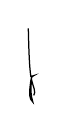
\begin{tikzpicture}[x=0.12cm,y=0.12cm]\draw[line width=0.45pt] (0,8) .. controls (0.05,6) and (0.10,4) .. (0.27,2.9) -- (0.60,3.0) .. controls (0.30,2.95) and (0.27,2.5) .. (0.22,2.1) .. controls (0.09,1.1) and (0.09,0.5) .. (0.48,0.2) .. controls (0.28,0.8) and (0.20,1.6) .. (0.36,2.5) .. controls (0.48,1.9) and (0.85,1.25) .. (0.58,0.9);\end{tikzpicture}}
une forme bil. alternée non dégénérée sur
\[
\varphi_\xi:M(A)\times M(A)\unsure{\mathbin{-}|\longrightarrow}T_\ell(\overline K^*)
\]
Alors
\[
\varphi_\xi(M^I,M_0^I)=0.
\]
En fait, les deux corollaires sont à priori équivalents, comme on constate aisément $\ldots\ldots$

\uline{Remarque} A la limite projective, \inserted{si $k$ est sép. clos,} les \unsure{hom|homo}
\[
\unsure{\alpha|\text{en}|\deleted{\ell^\nu}}\qquad {}_{\unsure{\ell^\nu}}A'(K)\times{}_{\ell^\nu}T(k)\to{}_{\ell^\nu}k^*\simeq{}_{\ell^\nu}K^*
\]
sont nuls. Cependant ces \unsure{accouplts|accouplements} eux mêmes ne
\margin{78}

\scanpage{80}
sont pas nuls en général $=$ pour $\nu=1$. En effet,
\inserted{supposons pour $A'$ la duale de $A$.}
si \deleted{$\unsure{x|\ell^\nu|\xi}$} $x\in{}_{\ell^\nu}T(k)$\inserted{$\subset{}_{\ell^\nu}A(K)\subset{}_{\ell^\nu}A(\overline K)$} est non nul, il existe un
$x'\in{}_{\ell^\nu}A'(\overline K)$ tel que \deleted{$\unsure{\varphi|\ell^\nu|\xi}$} $\varphi(x,x')\ne0$, et \deleted{\unsure{qui}} quitte
à agrandir $K$ en $K'$, on aura donc un
accouplement ${}_{\ell^\nu}A'(K)\times{}_{\ell^\nu}T(k)\longrightarrow{}_{\ell^\nu}k^*$ non nul .... :
\margin{79}

\scanpage{81}
\deleted{
\uline{Théorème}\quad $V$ anneau de val discrète\inserted{str. hensélien}, corps fr. $K$, corps rés. $k$,

$A$ schéma abélien sur $K$, modèle Néron $G$

$A'$ $\rule{2.6cm}{0.3pt}$ dual, $\rule{2.6cm}{0.3pt}$ $G'$

\deleted{$A_k$} $\overline K/K$,\quad $T_\ell(A(\overline K))$
\margin{$T$ \unsure{tor.|tore} maximal de $G_k$\\
$T'$ $\rule{2.6cm}{0.3pt}$ $G_k$,}
\[
\begin{aligned}
\underset{\begin{smallmatrix}\Vert\\M\end{smallmatrix}}{T_\ell(A(\overline K))}&\supset T_\ell(A(\overline K))^I
=T_\ell(A(\overline K)^I)=T_\ell(A(K))=T_\ell(G(V))
=\deleted{\unsure{T_\ell(G)}}\\
&=T_\ell(G(k))\unsure{=|\simeq}T_\ell(G^0(k))\supset T_\ell(T(k))
\end{aligned}
\]
\[
\begin{aligned}
M&\supset M^I\supset M^I_0\qquad\text{\unsure{du|de}. }=\\
M'&\supset M'^I\supset M'^I_0
\end{aligned}
\]
On
\[
M\times M'\xrightarrow{\varphi}T_\ell(\mathbb G_m(\overline K))=T_\ell(\overline K^*)
\left[\overset{\begin{smallmatrix}\text{\unsure{non}}\\\text{can}\end{smallmatrix}}{\simeq}\mathbf Z_\ell\right]
\]
je dis que
\[
\begin{cases}
\varphi(M^I_0,M'^I)=0\\
\varphi(M^I,M'^I_0)=0
\end{cases}
\]
\uline{Dém}\quad Pour simplifier, supposons \deleted{$\unsure{\ell|k}$} ${}_\ell G_k\subset G^0_k$.
\margin{\unsure{$r$|$\ell$}}
\[
V=\varinjlim A_i,\quad A_i\inserted{\subset V}\text{ de t.f. sur }\mathbf Z,\text{ \unsure{cont\textsuperscript{t}|contenant|contient} }t,\text{ uniformis.}
\]
$G$ \unsure{provient|pr\rule{1.3cm}{0.3pt}} de $G_i$, $G'$ de $G'_i$.

$T$ de $T_i$, $T'$ de $T'_i$

\deleted{On peut supposer que ${}_\ell G$.}
\[
\deleted{\unsure{X_i|\ell G}}\quad X_i=\unsure{\operatorname{Sp}|\operatorname{Spec}}(A_i),\quad Y_i=V(\unsure{t|\ell}\unsure{\mathcal O_{X_i}|\mathscr O_{X_i}}),\quad U_i=X_i-Y_i=X_{i\,t},
\]
\[
\begin{aligned}
{} _\ell G(k)&=\varinjlim {}_\ell G_i(Y_i),\\
{} _\ell G'(k)&=\unsure{\underline{\lim}|\varinjlim}{}_\ell G'_i(Y_i)
\end{aligned}
\]
\margin{On peut supposer $Y_i$ connexe, donc les \unsure{morphismes} de transition injectifs. Pour $i$ grand, ils sont bijectifs.}
\[
\begin{aligned}
{} _\ell G(k)&\simeq{} _\ell G_i(Y_i)&\qquad&\Big|\ {}_\ell T\\
{} _\ell G'(k)&={} _\ell G_i(Y'_i)&\qquad&\big|
\end{aligned}
\]
}
\margin{80.}

\scanpage{82}
\deleted{\unsure{É|E}xtensions et biextensions \unsure{de|des} \unsure{grpes|groupes} algébriques} \unsure{\deleted{\inserted{\unsure{abstrait|obstruct|obstruent}}}|\inserted{\unsure{abstrait|obstruct|obstruent}}} \deleted{par \unsure{$G_m$|des}}

Autodualité de la Jacobienne, suivant Artin-Mazur.
\margin{81}

\scanpage{83}
\uline{Cas de dim. relative} 1

Supposons \deleted{\unsure{$P\to$|que}} $X$ coh. plat/$S$ en dim $0$ i.e. $\mathrm H^0(X_s,\mathcal O_{X_s})\simeq k(s)$.

Posons $P'=\operatorname{Ker}(P\xrightarrow{\deg}\mathbf Z_S)$\qquad $Q'=\operatorname{Ker}(Q\xrightarrow{\deg}\mathbf Z_S)$

On a un diagramme commutatif de suites exactes de faisceaux fppf
\diagram{\begin{tikzcd}
&0\arrow[d]&0\arrow[d]&0\arrow[d,no head]&\\
0\arrow[r,no head]&\Phi\arrow[r]\arrow[d]&P^0\arrow[r]\arrow[d]&Q^0\arrow[r,no head]\arrow[d,no head]&0\\
0\arrow[r]&E\arrow[r]\arrow[d]&P'\arrow[r]\arrow[d]&Q'\arrow[r]\arrow[d]&0\\
0\arrow[r]&E/\Phi\arrow[r]\arrow[d]&E^*\arrow[r]\arrow[d]&\Psi\arrow[r]\arrow[d]&0\\
&0&0&0&
\end{tikzcd}}
$E,E^*,\Phi,\Psi$ sont \deleted{des \unsure{schémas en gr.}}\inserted{loc. ét (sur $S$)} représentables par des schémas en groupes \uline{étales}. Leurs fibres \unsure{génériques|générique} est le groupe unité. Les fibres spéciales, si $K(s)$ sep. clos, sont données par
\[
\Phi_{(s)}=\operatorname{Ker}u\simeq\mathbf Z/d\mathbf Z,\qquad
\Psi_{(s)}=\operatorname{Coker}u\qquad(d=\operatorname{pgcd}(d_i))
\]
où
\[
u:E_{(s)}\longrightarrow E^*_{(s)}
\]
est l'hom \unsure{compris|composé} \unsure{du|en} diagramme.
\diagram{\begin{tikzcd}
0\arrow[r]&\mathbf Z\arrow[r,"\lambda=(d_i)"]&\mathbf Z^r\arrow[r,"\alpha"]&E_{(s)}\arrow[r]\arrow[d,dashed,"u"]&0\\
\deleted{\unsure{0}}&\mathbf Z\arrow[l,draw=none,"\deleted{\longleftarrow}" description]&\mathbf Z^r\arrow[l,"\mu:(d_i\delta_i)=(d_i^t)"']&E^*_{(s)}\arrow[l,"\beta"']&0\arrow[l]
\end{tikzcd}}
et
\[
(\beta u\alpha)((n_i)_i)=\left(\sum_{1\le i\le r}n_i(C_i,C_j)/\delta_j\right)_{1\le j\le r}
\]
\margin{On a, si $X_{\widetilde S}$ est loc. \unsure{fact.|f.s.}}
\margin{\begin{tabular}{|p{2cm}}\hline
N.B. $E(s)\xleftarrow{\sim}E(S)\longrightarrow P'(S)$ est donné pr son composé avec $\alpha$, qui est $(n_i)\longmapsto\operatorname{cl}\underline O_X(\sum n_i C_i)$

$P'(S)\longrightarrow E^*_{(s)}\xleftarrow{\sim}E^{\unsure{*|\alpha}}(S)$ est donné pr son \unsure{composé|compos.} avec $\beta$, qui est $\underline L\longmapsto((\deg_{\unsure{k(s)}}\underline L_{C_i})/\delta_i)_i$.
\\\hline\end{tabular}}
\deleted{Lorsque $X$ \unsure{verifie|vérifie} $N$, alors $\Psi_{(s)}$ \unsure{est aussi|est} un groupe fini}

Si \deleted{$k(s)$ \unsure{est} \unsure{parfait} ou $(d^t,p)\unsure{=|-}1$, $\unsure{Q'|P'}$ \unsure{$\simeq$|est} \unsure{et|le}} les anneaux locaux de $X_{\widetilde S}$ factoriels, alors \unsure{$\Psi_{\inserted{s}\deleted{\unsure{(s)}}}$|$\Psi_{\inserted{s}}$ \deleted{\unsure{est}}} est aussi un groupe fini\inserted{(comme $\Phi_s$)},
\deleted{Si de plus les anneaux locaux de $X_s^{\sim}$ sont factoriels \unsure{p.ex.|puisque} $\unsure{V}$ \unsure{sur} $\unsure{S}$, alors}
\inserted{Si de plus\unsure{.} $K(s)$ est parfait \uline{ou} $(d^t,p)=1$,}\deleted{et}\inserted{alors}
$Q'$ est un modèle de Néron de
\[
Q'_\eta=P'_\eta=P^0_\eta=\underline{\operatorname{Pic}}^0_{X_\eta/K(\eta)}.
\]
En particulier, si $d^{\unsure{t|b}}=1$, donc $\Phi=0$, $Q'$ est un modèle de Néron de $\unsure{P^0_\eta|Q^0_\eta}$, \unsure{enfin} $P'$ est (loc ét) sur $S$ représentable.
\margin{82}

\scanpage{84}
NB. Accouplons $\mathbf Z^r$ et $\mathbf Z^r$ par
\[
((n_i),(n'_i))=\sum\delta_i n_i n'_i
\]
Alors $\lambda$ et $\mu$ sont formellement transposés par cet accouplement,
\deleted{\unsure{parfait}}, donc $\operatorname{Ker}\mu\simeq E^*(s)$ est accouplé à $\operatorname{Coker}\lambda\simeq E(s)$, par la formule
\[
(\alpha(x),y^*)=(x,\beta y^*)\qquad x\in\deleted{\unsure{E(s)|E_{(s)}}}\inserted{\mathbf Z^r},\ y^*\in E^*(s).
\]
\[
E(s)\times E^*(s)\longrightarrow\mathbf Z
\]
\deleted{Par suite,}\inserted{Je dis que} l'on a aussi
\[
(x,u(y))=(y,u(x))\qquad\text{pour }x,y\in E(s)
\]
En effet, on peut supposer que
\[
x=\alpha(\underbrace{(n_i)}_{\underline n}),\quad y=\alpha(\underbrace{(n'_j)}_{\underline n'}),
\]
et les deux mbs sont resp.
\[
\begin{aligned}
(\alpha(\underline n),u(y))&=(\underline n,\beta u\alpha(\underline n'))\\
(\alpha(\underline n'),u(x))&=(\underline n',\beta u\alpha(\underline n))
\end{aligned}
\]
Or on a
\[
(\underline n,\beta u\alpha(\underline n'))=\sum n_i n'_j(C_i C_j)
\]
qui est bien symétrique en \deleted{\unsure{$\in$|et}} $\underline n,\underline n'$.

Si les $\delta_i$ sont tous $1$, \inserted{(p.ex $k(s)$ p-fait)} alors on trouve \unsure{pr|pour|par} l'accouplement précédent
\[
E^*(s)\simeq\operatorname{Hom}(E(s),\mathbf Z)
\]
et la relation symétrique si on a de plus $d=1$ i.e. $d^t=1$.
Dans ce cas cette dualité, et le fait que $u:E(s)\unsure{\relbar\joinrel\relbar|\longrightarrow}E^*(s)$ \unsure{:} est autoadjoint, donne pour le $\operatorname{Coker}u=\Psi(s)$ une \uline{autodualité} canonique (à valeurs dans $\mathbf Q/\mathbf Z$).
Cette autodualité \deleted{\unsure{est liée à}}\inserted{exprime} l'obstruction à étendre la biextension qu'on a de $(Q'_\eta\times Q'_\eta)=(P^0_\eta\times P^0_\eta)$ par $G_{m\eta}$, par une biextension de $Q',Q'$\margin{modèles de Néron} par $G_m$
\margin{83}

\scanpage{85}
\begin{center}
INSTITUT\\
DES HAUTES ETUDES SCIENTIFIQUES\\
91 - BURES-SUR-YVETTE\\
928 48·53
\end{center}
\margin{84.}
